\documentclass[tikz,border=8pt]{standalone}
\usepackage{amsmath}
\usetikzlibrary{arrows.meta,positioning,fit,backgrounds,calc}

\definecolor{inputblue}{HTML}{DCEEFF}
\definecolor{encoderpurple}{HTML}{E7DDF5}
\definecolor{headpink}{HTML}{F7D9E3}
\definecolor{temporalgreen}{HTML}{DDF2E1}
\definecolor{featureyellow}{HTML}{FFF0C7}
\definecolor{policyorange}{HTML}{FAD9B8}
\definecolor{safetyred}{HTML}{F5C7C7}
\definecolor{outputblue}{HTML}{D5E8F6}
\definecolor{mutedgray}{HTML}{EEEEEE}

\tikzset{
  box/.style={draw, rounded corners=2pt, align=center, minimum height=9mm,
    minimum width=29mm, font=\small, line width=.65pt},
  smallbox/.style={box, minimum width=25mm, minimum height=8mm, font=\footnotesize},
  flow/.style={-{Latex[length=2.2mm]}, line width=.75pt},
  dataflow/.style={flow, draw=black!75},
  optional/.style={flow, dashed, draw=black!50},
  group/.style={draw=black!45, rounded corners=4pt, inner sep=5pt, dashed},
  labelnote/.style={font=\scriptsize, text=black!65, align=center}
}

\begin{document}
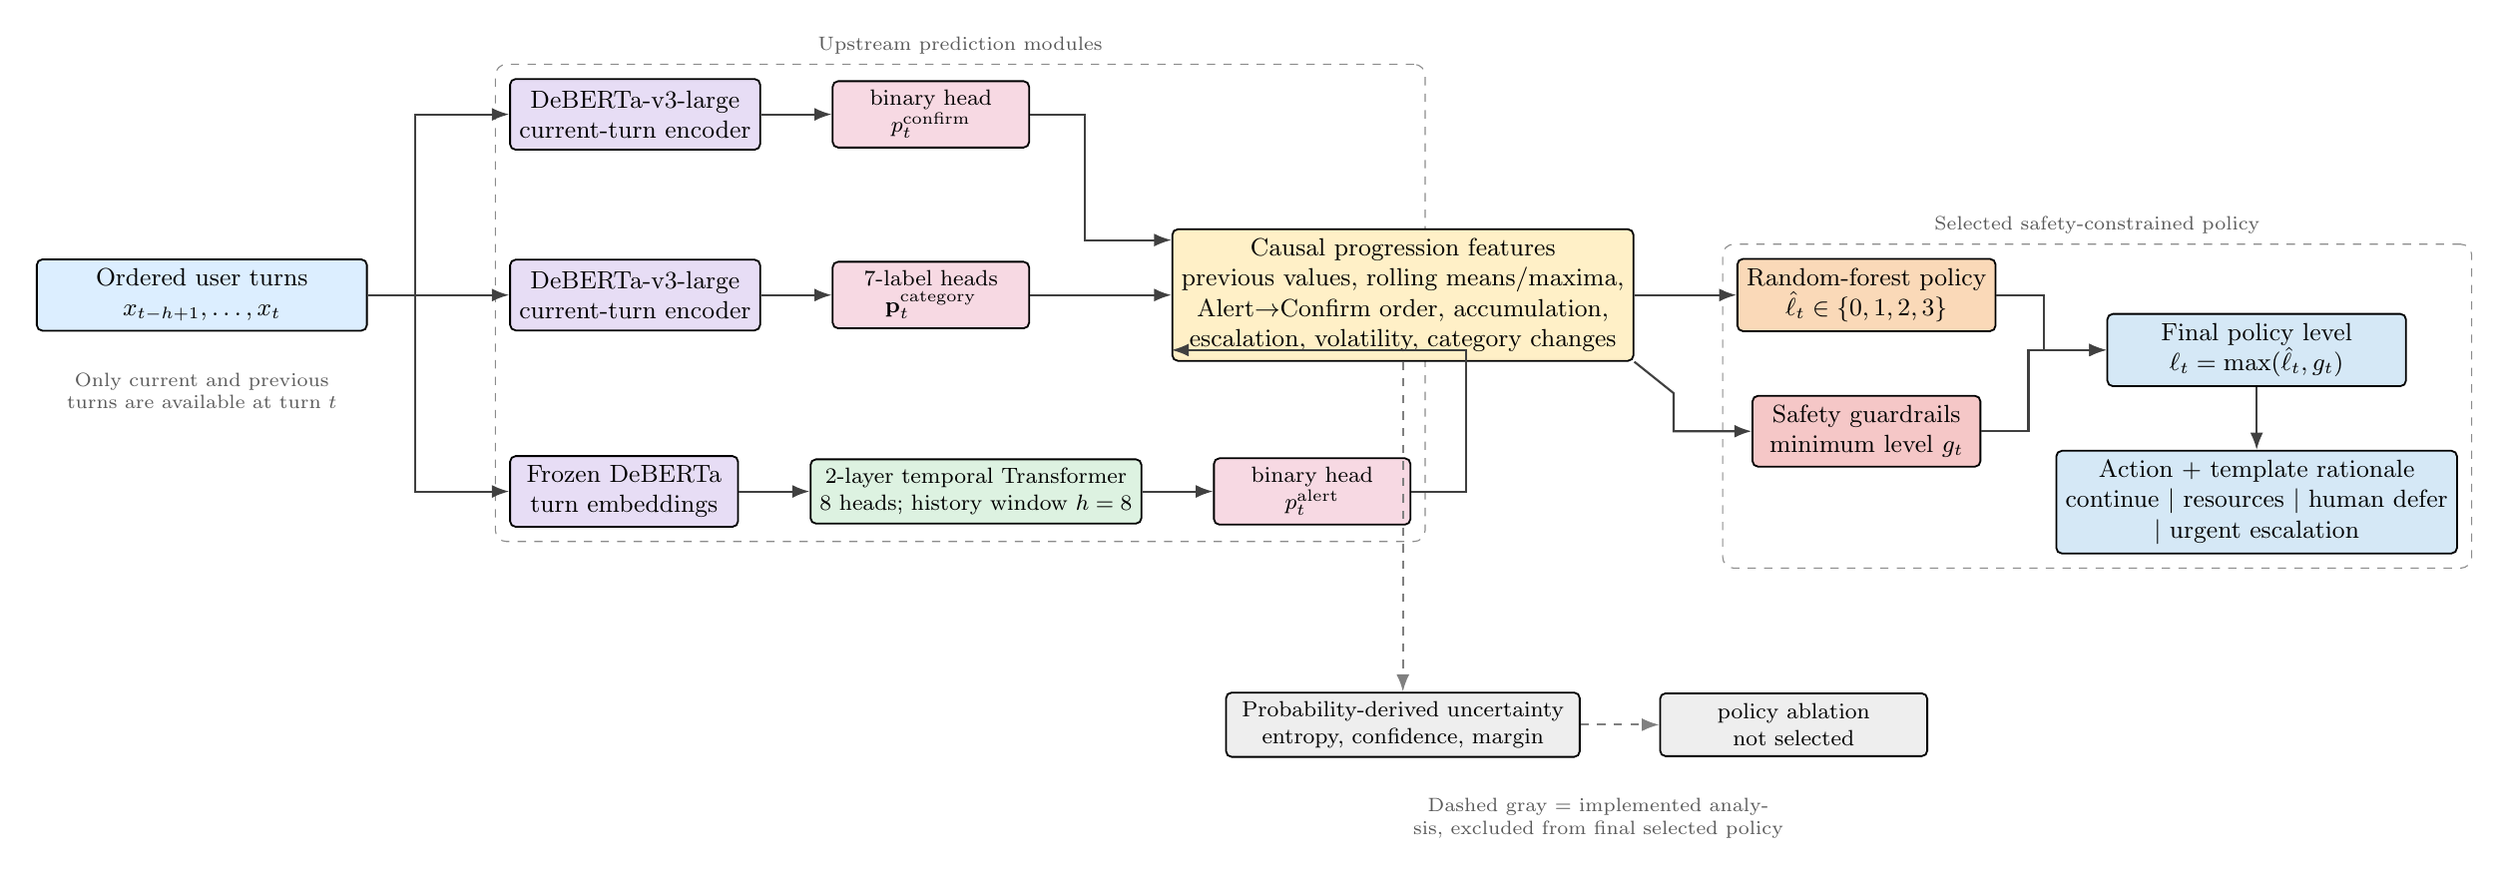
\begin{tikzpicture}[node distance=7mm and 9mm]

% Inputs
\node[box, fill=inputblue, minimum width=42mm] (turns)
  {Ordered user turns\\$x_{t-h+1},\ldots,x_t$};

% Neural branches
\node[box, fill=encoderpurple, right=18mm of turns, yshift=23mm] (confirmenc)
  {DeBERTa-v3-large\\current-turn encoder};
\node[smallbox, fill=headpink, right=of confirmenc] (confirmhead)
  {binary head\\$p_t^{\mathrm{confirm}}$};

\node[box, fill=encoderpurple, right=18mm of turns] (catenc)
  {DeBERTa-v3-large\\current-turn encoder};
\node[smallbox, fill=headpink, right=of catenc] (cathead)
  {7-label heads\\$\mathbf p_t^{\mathrm{category}}$};

\node[box, fill=encoderpurple, right=18mm of turns, yshift=-25mm] (embed)
  {Frozen DeBERTa\\turn embeddings};
\node[smallbox, fill=temporalgreen, right=of embed] (temp)
  {2-layer temporal Transformer\\8 heads; history window $h=8$};
\node[smallbox, fill=headpink, right=of temp] (alerthead)
  {binary head\\$p_t^{\mathrm{alert}}$};

\draw[dataflow] (turns.east) -- ++(6mm,0) |- (confirmenc.west);
\draw[dataflow] (turns.east) -- (catenc.west);
\draw[dataflow] (turns.east) -- ++(6mm,0) |- (embed.west);
\draw[dataflow] (confirmenc) -- (confirmhead);
\draw[dataflow] (catenc) -- (cathead);
\draw[dataflow] (embed) -- (temp);
\draw[dataflow] (temp) -- (alerthead);

% Progression and policy
\node[box, fill=featureyellow, minimum width=47mm, right=18mm of cathead] (features)
  {Causal progression features\\previous values, rolling means/maxima,\\Alert$\rightarrow$Confirm order, accumulation,\\escalation, volatility, category changes};

\draw[dataflow] (confirmhead.east) -- ++(7mm,0) |- ([yshift=7mm]features.west);
\draw[dataflow] (cathead.east) -- (features.west);
\draw[dataflow] (alerthead.east) -- ++(7mm,0) |- ([yshift=-7mm]features.west);

\node[box, fill=policyorange, right=13mm of features] (rf)
  {Random-forest policy\\$\hat\ell_t\in\{0,1,2,3\}$};
\node[box, fill=safetyred, below=8mm of rf] (guard)
  {Safety guardrails\\minimum level $g_t$};
\node[box, fill=outputblue, right=14mm of rf, yshift=-7mm, minimum width=38mm] (final)
  {Final policy level\\$\ell_t=\max(\hat\ell_t,g_t)$};
\node[box, fill=outputblue, below=8mm of final, minimum width=43mm] (actions)
  {Action + template rationale\\continue $\mid$ resources $\mid$ human defer\\$\mid$ urgent escalation};

\draw[dataflow] (features) -- (rf);
\draw[dataflow] (features.south east) -- ++(5mm,-4mm) |- (guard.west);
\draw[dataflow] (rf.east) -- ++(6mm,0) |- (final.west);
\draw[dataflow] (guard.east) -- ++(6mm,0) |- (final.west);
\draw[dataflow] (final) -- (actions);

% Unselected uncertainty branch: placed on a separate row to avoid the Alert path.
\node[smallbox, fill=mutedgray, below=42mm of features, minimum width=45mm] (uncert)
  {Probability-derived uncertainty\\entropy, confidence, margin};
\node[smallbox, fill=mutedgray, right=10mm of uncert, minimum width=34mm] (ablation)
  {policy ablation\\not selected};
\draw[optional] (features.south) -- ++(0,-7mm) -| (uncert.north);
\draw[optional] (uncert) -- (ablation);

% Group labels
\begin{scope}[on background layer]
  \node[group, fit=(confirmenc)(confirmhead)(catenc)(cathead)(embed)(temp)(alerthead),
    label={[labelnote]above:Upstream prediction modules}] {};
  \node[group, fit=(rf)(guard)(final)(actions),
    label={[labelnote]above:Selected safety-constrained policy}] {};
\end{scope}

\node[labelnote, text width=42mm, below=4mm of turns]
  {Only current and previous turns are available at turn $t$};
\node[labelnote, text width=78mm, anchor=north]
  at ($(uncert.south)!0.5!(ablation.south)+(0,-4mm)$)
  {Dashed gray = implemented analysis, excluded from final selected policy};

\end{tikzpicture}
\end{document}
